%!TEX root = ../memoire.tex

\chapter{Adaptation de GenDR}\label{ch:implementation}

Au chapitre précédent, nous avons expliqué comment nous avons extrait les informations de VerbNet à l'aide de scripts Python pour nous en servir dans GenDR. Ce chapitre couvrira l'adaptation de GenDR pour lui faire exploiter ces nouvelles données. D'abord, nous expliquerons comment nos dictionnaires fonctionnent après l'importation de VerbNet et comment ils communiquent entre eux. Puis, nous allons montrer comment fonctionnent les nouvelles règles de grammaire qui activent ces connaissances lexicales.

\section{Adaptation des dictionnaires}

Au chapitre \ref{chapgendr}, nous avons montré comment le lexique s'encodait dans GenDR. Nous avions deux dictionnaires: un dictionnaire de sémantèmes (\emph{semanticon}) et un dictionnaire de lexèmes (\emph{lexicon}). À la suite des informations extraites sur les \acp{GP}, nous avons maintenant un dictionnaire de \acp{GP} (\emph{gpcon}), ce qui implique un changement important de l'architecture du \emph{lexicon} et des règles de la grammaire.

\subsection{Une nouvelle architecture pour le \emph{lexicon}}

Comme nous l'avons vu à la section \ref{sec:dictio}, GenDR listait et décrivait les comportements syntaxiques des verbes directement dans le \emph{lexicon}, qu'on a maintenant séparé en quatre sections: les classes abstraites, les verbes de VerbNet, les classes verbales de VerbNet et le reste du lexique .

La première section, \textbf{\texttt{ABSTRACT CLASSES}}, décrit les classes générales de GenDR. Elle donne les propriétés génériques des verbes, noms, noms propres, adjectifs, montants, etc. Anciennement, on avait une hiérarchie rudimentaire de classes de verbes (intransitif, transitif direct/indirect et ditransitif) comprenant toute l'information syntaxique pour chaque sous-classe. Maintenant, la classe générale \texttt{VERB} ne contient que les informations partagées par tous les verbes du dictionnaire: sa partie du discours profonde et celle de surface. Les autres catégories syntaxiques comme les noms ou les adjectifs contiennent plus d'information que la classe générale \texttt{VERB}. Puisque leurs comportements sont prédictibles, contrairement aux verbes, on encode, en plus de la partie du discours, un patron de régime par défaut et des traits morpho-syntaxiques lorsque c'est nécessaire. Par contre, comme vous pouvez le voir dans la classe \texttt{NOUN}, on n'a pas l'information syntaxique explicite que donnent les patrons de régime, on n'a que l'identifiant de celui-ci. Les propriétés de chaque patron de régime sont encodées dans le dictionnaire prêt à cet effet (\emph{gpcon}).

\begin{lstlisting}[language=mate, caption = Extrait du \emph{lexicon}: attributs par défaut des classes génériques, label=classedef]
/*
=======================================================
                  ABSTRACT CLASSES
=======================================================
*/

// ================= VERBS =================

// VERB
// ----

verb {
  dpos = V
  spos = verb
}

// ================= NOUNS =================

// NOUN
// ----
// Common nouns.

noun {
  dpos = N
  spos = noun
  countable = yes
  gp = { id=NP dia=1}
}
...
\end{lstlisting}

La deuxième section, \textbf{\texttt{VERBNET MEMBERS}}, contient les membres des classes verbales de VerbNet que nous avons extraits (voir figure~\ref{scriptmember}). Sont ici listés tous les 6\,393 verbes, ainsi que la classe de VerbNet (ou la sous-classe) à laquelle ils appartiennent. Dans cette section, on distingue les différentes acceptions d'un vocable en fonction de la classe qui lui est associée. Par exemple, pour la forme \form{order}, on a \texttt{order\_1 : "get-13.5.1"} (\sem{passer une commande}) et \texttt{order\_2 : "order-60-1"} (\sem{donner un ordre}).

\begin{lstlisting}[language=mate, caption = Extrait du \emph{lexicon}: unités lexicales verbales]
/*
 =======================================================
                      VERBNET MEMBERS
 =======================================================
*/
"open up" : "establish-55.5-1"
operate : "other_cos-45.4"
oppose : "amalgamate-22.2-3"
ordain : "appoint-29.1"
order_1 : "get-13.5.1"
order_2 : "order-60-1"
organize_1 : "create-26.4"
organize_2 : "establish-55.5-1"
organize_3 : "force-59-1"
originate : "establish-55.5-1"
ornament_1 : "butter-9.9"
ornament_2 : "fill-9.8"
ornament_3 : "illustrate-25.3"
...
\end{lstlisting}
\draft{

La troisième section, \textbf{\texttt{VERBNET CLASSES}}, liste les types de \acp{GP} que sélectionne chaque classe verbale. Cela se modélise par un trait \texttt{gp} dont la valeur est une structure qui contient deux attributs: la diathèse (\texttt{dia}) et l'identifiant du patron de régime (\texttt{id}). La diathèse d'un \ac{GP} s'encode ainsi différement dans le nouveau \emph{lexicon}. Anciennement, la diathèse était explicitée dans l'entrée \texttt{prédicate}, qui donnait une diathèse triviale par défaut à tous les prédicats du dictionnaire, mais qu'on pouvait court-circuiter pour un lexème donné. Maintenant, on spécifie pour chaque \ac{GP} la diathèse qui lui est associée de cette manière: \texttt{dia=132}\FL{faut utiliser une convention typographique pour les éléments de code, à revoir} (ça implique \texttt{I:1 II:3 III:2}). Autrement dit, l'ordre de présentation des actants sémantiques (les chiffres arabes 1,3,2) correspondra à la réalisation syntaxique de ces actants (I,II,III). Puis finalement, chaque classe verbale est dotée d'un trait \texttt{id} qui permettra au système de récupérer les propriétés syntaxiques de cet identifiant dans le dictionnaire de patrons de régime. Nous les avons encodé manuellement les uns après les autres grâces aux phrases exemples pour déduire la diathèse de chaque patron puisqu'elle n'est pas explciité par VerbNet. et parce que les rôles th/vs en syntx ne nous donne rien.

Toutefois, nous avons relevé un problème important après avoir manuellement encodé chaque diathèse. Il se trouve que le mécanisme d'héritage que nous postulions ne transmet pas toutes les informations que nous désirions qu'il transmette. La partie du discours est héritée sans problème, mais les patrons de régime ne le sont pas. C'est une erreur de notre part que nous avons remarqué en faisant quelques tests après avoir préparé notre dictionnaire. Ainsi, nous avons dû manuellement les rajouter de chaque classe mère à chaque classe fille parce que les patrons ne se transmettaient pas. Le problème provient du fait que l'architecture que nous avons instauré bloque l'héritage \draft{il faudrait que tu me réexpliques brièvement pourquoi ça bloque, c'est parce qu'on le redéfini et il perd ses propriétésé précédentes ?} puisqu'on redéfini l'attribut gp au complet à chaque fois. Ainsi, le système ne peut récupérer que les gps encodés dans la classe et ne peut pas récupérer l'attribut gp dans les classes dominantes. Cependant,  Le trait dpos a pu se transmettre de sous-classes, en classes jusqu'à la classe abstraite, mais c'est parce que le trait dpos n'est jamais redéfini qu'il a pu monté ainsi. 

Comme nous avions déjà manuellement écrit la diathèse de chaque \ac{gp}, nous n'avons donc pas pu corriger la situation en modifiant le script python pour que les patrons des classes mères soient automatiqument transmis aux classes filles. Il aurait quand même fallu prendre le temps de réécrire manuellement les diathèses dans le lexicon. Nous l'avons donc corrigé manuellement, autrement dit nous avons inséré les patrons de régime des classes mères dans les classes filles. Toutefois, ç'aurait pu être fait automatiquement si nous n'avions pas déjà commencé à analyser les patrons de régime pour leur accorder la bonne diathèse. Puisque celle-ci n'a pas pu être extraite de VerbNet, comme ils ne l'encodent pas de cette manière. Ils utilisent les rôles thématiques pour faire le passage des rôles sémantiques aux constituants syntaxiques. L'inconvénient de cette situation est que notre dictionnaire est maintenant beaucoup plus fourni qu'il ne l'était, mais au moins nous respectons l'architecture que VerbNet avait établi.

Toutefois, ce mécanisme fonctionne très bien pour d'autres but, il est utilisé pour que chaque membre verbal correspondant à une classe donnée hérite des patrons de régime de celle-ci. Dans ces cas, l'héritage se fait très bien puisque la valeur gp n'est jamais redéfinie dans chaque membre. Cela nous évite de donc de surpeupler notre système, puisque la description de 6\,394 verbes saturerait notre dictionnaire d'information.}

\begin{lstlisting}[language=mate, caption = Extrait du \emph{lexicon}: classes de VerbNet, label=fig:vnclass]
/*
=======================================================
                   VERBNET CLASSES
=======================================================
*/

"tell-37.2": verb {
  gp = { id=NP_V_NP  
	       dia=12 } // John informed me.
  gp = { id=NP_V_NP_PP_of_topic  
	       dia=123 } // John informed me of the situation. }

"tell-37.2-1": "tell-37.2" {
  gp = { id=NP_V_NP  
	       dia=12 } // John informed me.
  gp = { id=NP_V_NP_PP_of_topic  
	       dia=123 } // John informed me of the situation. }
  gp = { id=NP_V_NP  
	       dia=12 } // Ellen told a story.
  gp = { id=NP_V_NP_PP_to_recipient 
		     dia=123 } // Ellen told a story to Helen.
  gp = { id=NP_V_NP_Dative_NP   
	       dia=132 } // Ellen told Helen a story.
  gp = { id=NP_V_NP
		     dia=13 } // Ellen told Helen.
  gp = { id=NP_V_NP_PP_about_topic
		     dia=132 } // Ellen told Helen about the situation. }
...
\end{lstlisting}

Passons ensuite à la section \texttt{NON-VERBAL LEXICAL ENTRIES} qui regroupe \textbf{le reste du lexique}: noms, adjectifs, adverbes, prépositions, déterminants, etc. Ces entrées proviennent de la version originale de GenDR \citep{lareau18} et le contenu de cette section a été enrichi par les lexèmes qu'on retrouvait dans les phrases exemples de VerbNet. Bref, les entrées de cette section pointent vers les classes (\texttt{NOUNS}, \texttt{PREPOSITIONS}, \ldots) abstraites leur correspondant, ce qui leur permet d'hériter des attributs suivants: \texttt{dpos},\texttt{spos}, \texttt{id}, et \texttt{dia}.

\begin{lstlisting}[language=mate, caption = Extrait du \emph{lexicon}: unités lexicales non-verbales]
/*
=======================================================
               NON-VERBAL LEXICAL ENTRIES     
=======================================================
*/
accountant : noun
acorn : noun
acquaitance  : noun
across : preposition
...
\end{lstlisting}

\subsection{Le dictionnaire des patrons de régime: \emph{gpcon}}

Le \emph{gpcon} est un dictionnaire de patrons de régime qui contient 278 identifiants uniques de \acp{GP} et leurs propriétés syntaxiques. Considérant que les classes verbales du lexicon partagent ces patrons de régime, l'option de les encoder dans un dictionnaire à part nous apparaît évidente. Cela allège grandement le contenu du lexicon et ça nous permet d'entretenir les données plus facilement. Ainsi, la modification d'un \ac{GP} dans le gpcon est donc appliqué à toutes les classes verbales utilisant ce gp. 

Une entrée typique dans ce dictionnaire contient: l'identifiant du \ac{GP} et ses propriétés syntaxiques qui sont explicitées par l'énumération des actants syntaxiques compris pour ce régime ainsi que les contraintes des actants (comme la partie du discours nécessaire à la lexicalisation). Nous avons aussi instauré un mécanisme pour tenir compte du fait que certains patrons de régime permettent deux prépositions en compétition pour le même actant syntaxique. C'est le cas par exemple pour le \ac{GP} \texttt{NP\_asset\_V\_NP\_PP\_from\_out\_of}, qui contient \lstinline|III={rel=oblique dpos=N prep=from}| et \lstinline|III={rel=oblique dpos=N prep="out of"}|. Ce mécanisme nous permet de mieux exploiter la richesse de combinatoire des verbes pour générer plus de paraphrases.

Cependant, ce dictionnaire n'est pas sans failles. Nous nous sommes rendu compte qu'il existait des doublons de \ac{GP} en termes de contenu. L'origine de ces doublons provient de VerbNet qui utilise des rôles thématiques pour identifier les actants syntaxiques, ce qui permet à deux \ac{GP} d'avoir des propriétés identiques mais des identifiants différents. Par exemple, les patrons \texttt{NP\_agent\_V} et \texttt{NP\_attribute\_V} couvrent la même construction, mais la différence provient du fait que l'actant syntaxique I est de type agentif et l'actant II est attributif. Nous avons gardé ces doublons puisqu'ils proviennent de l'architecture de VerbNet et ils pourraient nous être utile si nous voulions faire le pont avec une autre ressource qui se sert des rôles thématiques pour identifier la diathèse.

\begin{lstlisting}[language=mate, caption = Extrait du \emph{gpcon}]
NP_agent_V {
   I={rel=subjective dpos=N}
}
NP_agent_V_NP {
   I={rel=subjective dpos=N}
   II={rel=dir_objective dpos=N}
}
NP_asset_V_NP_PP_from_out_of {
   I={rel=subjective dpos=N}
   II={rel=dir_objective dpos=N}
   III={rel=oblique dpos=N prep=from}
   III={rel=oblique dpos=N prep="out of"}
}
NP_attribute_V {
   I={rel=subjective dpos=N}
}
...
\end{lstlisting}

\section{Adaptation de la grammaire}

Les modifications apportées aux dictionnaires entraînent des modifications dans les règles de la grammaire. Nous les présenterons dans la section suivante. En ce qui concerne le module sémantique, l'essentiel de la version originale de GenDR a été transposée, mais nous avons dû façonner quelques nouvelles règles pour tenir compte de l'intéraction entre les identifiants des patrons de régime dans le lexicon et leur description syntaxique dans le gpcon.

\subsection{Module sémantique}

Dans le chapitre \ref{chapgendr}, nous avons démontré comment fonctionnait l'arborisation et la lexicalisation dans GenDR, nous démontrerons maintenant comme ceux-ci intéragissent dans la nouvelle version.

\textbf{L'arborisation} et la \textbf{lexicalisation} (cf. \ref{sec:arbo},\ref{sec:lexicalisation}) reprennent des règles de la version originale et en ajoute des nouvelles pour tenir compte de l'implémentation de VerbNet dans GenDR. Nous énumérerons donc les étapes nécessaires pour le passage de la \ac{RSem}--\ac{RSyntP} dans la nouvelle version de GenDR.

\begin{enumerate}
  \item \textbf{Création de la racine}.
  L'application de la règle \emph{root\_standard} n'a pas changé, donc on construit la racine de l'arbre syntaxique à partir du \ac{ND} de la structure sémantique.

  \item \textbf{Lexicalisation de la racine}.
  Comme dans l'ancienne version, on applique une règle de lexicalisation pour trouver dans les dictionnaires pour trouver un lexème qui correspondra au sens demandé tout en respectant les contraintes imposées. Toutefois, malgré que cette étape reste identique, la nouvelle version de GenDR sollicitera beaucoup plus une règle de lexicalisation de secours pour réaliser la racine puisque les 6\,394 verbes de GenDR ne figurent pas tous dans le semanticon. Toutefois, comme ils sont désambiguïsés, il s'agit généralement d'un ration 1:1 entre un lexème désambiguïsé et son sens correspondant. Bref, la règle de lexicalisation de secours va s'appliquer puisque le sémantème de la racine ne figure pas dans le semanticon, mais il existe dans le lexicon, donc le système supposera que le lexème dans le dictionnaire correspond au signifié du sémantème dans la structure d'input.

  \item \textbf{Sélection du patron de régime}.
  Une fois que le n\oe{}ud racine est lexicalisé, la règle \emph{actant\_gp\_selection} est déclenchée, ce qui permet à GenDR de récupérer les informations encodées dans l'entrée lexicale correspondant à la racine, par exemple, si la racine est lexicalisée comme \lex{order\_1}, alors le système parcoure le dictionnaire pour trouver ce membre verbal: \lstinline|order_1 : "get-13.5.1"|. Ensuite, le mécanisme d'héritage permet au lexème \lex{order\_1} d'hériter du trait \texttt{gp} qui renferme les informations \texttt{id} et \texttt{dia} de la classe \texttt{get-13.5.1}. Celles-ci sont ainsi récupérées par la règle et apposé sur la racine lexicalisée. Cette règle peut ainsi mener à la construction de plusieurs arbres profonds puisque le système génère autant de racine qu'il y a de traits \texttt{gp}, mais seuls ceux qui respectent les contraintes qui suivront génèreront réellement des arbres, les autres resteront incomplets.
	
	\item \textbf{Application d'une règle actancielle}.
	À l'étape précédente, le n\oe{}ud racine de l'arbre profond était enrichi des traits \texttt{id} et \texttt{dia} qui sont essentiels à l'application des règles actancielles. Il existe ainsi jusqu'à six versions de cette règle actancielle, ce qui permet à un prédicat de sélectionner jusqu'à six actants sémantiques. Le maximum que nous avons dans ce dictionnaire est quatre actants sémantiques, mais nous voulions tenir compte de toutes les possibilités. Ce mécanisme est donc nouveau puisque dans l'ancienne version de GenDR, le système analysait chaque liaison actancielle individuellement, puis la faisait correspondre à une relation syntaxique. Cela se traduisait par la création d'un arc entre la racine et un n\oe{}ud vide qui se faisait imposer des contraintes par son gouverneur (la racine dans ce cas). La version actuelle de GenDR ne fonctionne plus ainsi, maintenant, le gp sélectionné déclenche une règle actancille en fonction du nombre d'actant compris dans sa diathèse, puis on crée des arcs en partance du gouverneur vers trois n\oe{}uds vides non-contraints.
	
	Bref, une règle actancielle est donc choisie en fonction de la diathèse qui est précisée par le trait \texttt{dia}. De plus, pour que l'arborisation se fasse correctement, il faut que les actants sémantiques se trouvant dans la diahtèse se retrouve dans la structure sémantique donnée. Sinon, l'application de la règle échoue. Cette règle va donc permettre l'application des gps satisfaisant les contraintes de diathèses. Ainsi, si trois patrons de régime pour une classe verbale s'exprime par les mêmes actants sémantiques, la règle actancielle s'appliquera pour chacun de ceux-ci et poursuivra l'arbre.
	
	\item \textbf{Application des contraintes sur les n\oe{}uds}
Notre avons décidé de créer une règle qui s'occupait strictement d'imposer les contraintes aux noeuds nouvellement créés par les règles actancielles. Bref, la règle récupère les restrictions sur les n\oe{}uds qui sont encodés comme propriétés syntaxiques des \acp{GP} dans le \emph{gpcon} (voir la figure~\ref{gpexemple}). La règle d'application de contraintes s'applique trois fois puisqu'il y a trois n\oe{}uds vides, qui sont maintenant contraints par tous les traits nécessaires comme la partie du discours ou la finitude (quand un verbe sélectionne un autre verbe).

	\item \textbf{Lexicalisation des n\oe{}uds contraints}
Ensuite, on répète la phase de lexicalisation, dans ce cas, il s'agit de \emph{lex\_standard} puisque tous les sémantèmes figurent dans le \emph{semanticon} et le \emph{lexicon}. Cette règle s'applique aussi trois fois car il y a trois n\oe{}uds. Si les propriétés des lexèmes \lex{teacher}, \lex{history} ou \lex{student} ne respectaient pas les contraintes du n\oe{}ud, alors la lexicalisation aurait échoué.

Puis, si les lexèmes qui viennent d'être lexicalisés déclencheront l'application de la règle 2 et si ces lexèmes sélectionnent des actants sémantiques, alors la règle 3 s'appliquera jusqu'à la règle 6 une seconde fois, et ainsi de suite jusqu'à ce que le parcours de la structure sémantique soit complété et cela résulte en la construction de l'arbre syntaxique profond.

\end{enumerate} 

\section{Exemple}

Pour notre exemple, nous verrons comment se réalise la phrase \form{The teacher talked about history to the students}. La figure~\ref{fig:history} représente la structure sémantique que nous avons donnée en input au système. Le n\oe{}ud dominant est \sem{talk\_3} et il lie 3 actants sémantiques: \sem{teacher}, \sem{student} et \sem{history}. Chaque n\oe{}ud reçoit les traits grammaticaux de temps, nombre et définitude appropriés.

\begin{lstlisting}[language=mate, caption=Structure sémantique de \form{The teacher talked about history to the students}, label=fig:history]
structure Sem S {
  S:1{
    talk_3:1{
      tense=PAST 
      1-> teacher:1
      2-> student:1
			3-> history:1
    }
    teacher:1{number=SG definiteness=DEF}
    history:1{number=SG definiteness=NO}
    student:1{number=PL definiteness=DEF}
    main-> talk_3:1
  }
}
\end{lstlisting}

Cet input permet de générer neuf structures syntaxiques profondes, qui correspondent aux phrases suivantes:

\begin{enumerate}
  \item \form{The teacher talked.}
  \item \form{The teacher talked to the students.}
  \item \form{The teacher talked with the students.}
  \item \form{The teacher talked to the students about history.}
  \item \form{The teacher talked with the students about history.}
  \item \form{The teacher talked about history to the students.}
  \item \form{The teacher talked about history with the students.}
  \item \form{Te teacher talked about history.}
\end{enumerate}
\draft{J'ai retiré un gp, puisqu'il s'agissait d'une incompatibilité TST-VerbNet et j'voulais pas rentrer dans les détails tout de suite.}

Bien que nous n'en visions qu'une en particulier, neuf réalisations ont découlé de l'application de cet input parce que \lex{talk\_3} appartient à la classe \texttt{"talk-37.5"} et en hérite les neuf patrons de régime associés. Toutes ces constructions ont pu être réalisées parce que les \acp{GP} satisfaisaient les contraintes demandées par l'input.

\begin{lstlisting}[language=mate, caption=Classe \texttt{talk-37.5} dans le \emph{lexicon}]
"talk-37.5": verb {
  gp = { id=NP_V
	       dia=1 } // Susan talked.
  gp = { id=NP_V_PP_to_co_agent
	       dia=12 } // Susan talked to Rachel.
  gp = { id=NP_V_PP_with_co_agent
	       dia=12 } // Susan talked with Rachel.
  gp = { id=NP_V_PP_to_co_agent_PP_about_topic
	       dia=123 } // Susan talked to Rachel about the problem.
  gp = { id=NP_V_PP_with_co_agent_PP_about_topic
	       dia=123 } // Susan talked with Rachel about the problem.
  gp = { id=NP_V_PP_about_topic_PP_to_co_agent
	       dia=132 } // Susan talked about the problem to Rachel.
  gp = { id=NP_V_PP_about_topic_PP_with_co_agent
	       dia=132 } // Susan talked about the problem with Rachel.
  gp = { id=NP_V_PP_about_topic
	       dia=13 } // Susan talked about the problems of modern America.
}
\end{lstlisting}

\FL{assure-toi que tes captions soient très explicites, parce que les lecteurs vont souvent juste sauter d'une figure à l'autre et lire le texte seulement s'ils ne comprennent pas la figure}

\begin{lstlisting}[language=XML, caption=Propriétés syntaxiques de \texttt{NP\_V\_PP\_about\_topic\_PP\_to\_co\_agent} , label=gpexemple]

NP_V_PP_about_topic_PP_to_co_agent {
   I={rel=subjective dpos=N}
   II={rel=oblique dpos=N prep=about}
   III={rel=indir_objective dpos=N prep=to}
	}
\end{lstlisting}

\subsection{Création et lexicalisation de la racine}
Application de la règle \emph{root\_standard} pour crééer la racine. Le sémantème \sem{talk\_3} n'existe pas dans le semanticon donc une règle de lexicalisation  s'occupe de vérifier dans le lexicon s'il existe un lexème correspondant, il trouve \lex{talk\_3} et en fait la lexicalisation de la racine.

\begin{figure}[htb]
	\centering
	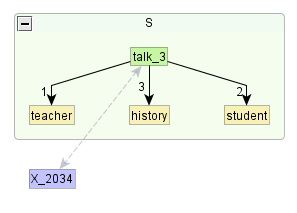
\includegraphics[width=0.4\textwidth, trim = {0cm 0cm 0cm 0cm},clip]{ch6/figs/root.png}
	\caption{Création de la racine à partir du n\oe{}ud dominant}
	\label{deroulement0}
\end{figure}


\subsection{Sélection du patron de régime dans le lexicon}
Ensuite, la règle \emph{actant\_gp\_selection} est déclenchée par l'apparition de \lex{talk\_3} pour satisfaire la racine. GenDR récupère les traits encodés pour chaque attribut \texttt{gp} de la classe verbale \texttt{talk-37.5}. Il récupère ensuite le trait\texttt{id} dont la valeur est \texttt{NP\_V\_PP\_about\_topic\_PP\_to\_co\_agent} et le \texttt{dia} dont la valeur est \texttt{132}. Puis, il appose ces traits sur la racine, car ils seront récupérés par les règles actancielles.

\begin{figure}[htb]
	\centering
	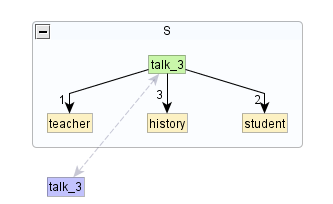
\includegraphics[width=0.4\textwidth, trim = {0cm 0cm 0cm 0cm},clip]{ch6/figs/selectiongp.png}
	\caption{Application de la règle actant\_gp\_selection}
	\label{deroulement1}
\end{figure}

\subsection{Application de la règle actancielle: \emph{actant\_gp\_ijk}}
La règle \emph{actant\_gp\_ijk} (ijk=3 actants) est sélectionnée puisque le trait de diathèse apposé sur le noeud précise qu'il y a trois actants sémantiques. À ce point-ci, pour que l'arborisation se fasse correctement, il faut que les actants sémantiques imposés par la diahtèse correspondent à ceux donnés par la structure sémantique. Comme notre exemple d'input en contient trois, alors la règle s'applique correctement et trois arcs en partance de la racine sont créés au bout desquels se trouvent des noeuds vides.

\begin{figure}[htb]
	\centering
	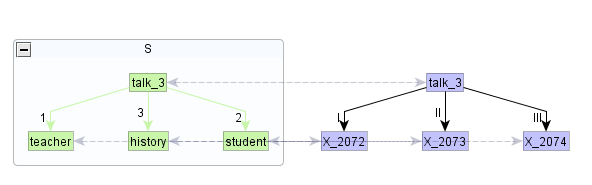
\includegraphics[width=1\textwidth, trim = {0cm 0cm 0cm 0cm},clip]{ch6/figs/actant_gp_ijk.png}
	\caption{Application d'une règle actancielle: actant\_gp\_ijk}
	\label{deroulement2}
\end{figure}

\subsection{Application des contraintes sur les n\oe{}uds}
La règle récupère les restrictions sur les actants syntaxiques que sélectionne talk-3-1.5, qui sont encodés dans le \emph{gpcon}: \lstinline|NP_V_PP_about_topic_PP_to_co_agent { I={rel=subjective dpos=N}, II=...| (voir \ref{gpexemple} ). Dans ce cas, la règle d'application de contraintes s'applique trois fois puisqu'il y a trois n\oe{}uds vides, qui sont maintenant contraints par tous les traits nécessaires.

\subsection{Lexicalisation des n\oe{}uds contraints}
On lexicalise tous les noeuds puisqu'ils en respectent les contraintes. Le système utilisera une règle de lexicalicasaion simple dans ce cas puisque chacun de ces sémantèmes existent dans le semanticon.

\begin{figure}[htb]
	\centering
	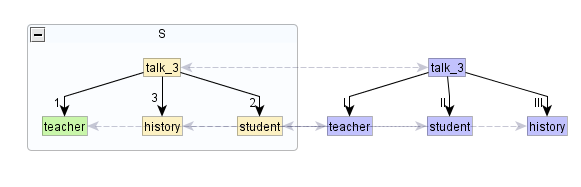
\includegraphics[width=1\textwidth, trim = {0cm 0cm 0cm 0cm},clip]{ch6/figs/lex.png}
	\caption{Applications d'une règle de lexicalisation: lex\_standard}
	\label{deroulement3}
\end{figure}

\subsection{Application de la règle \emph{actant\_gp\_selection}}
Finalement, la règle \emph{actant\_gp\_selection} est sollicitée pour les trois noeuds nouvellement lexicalisés \lex{teacher},\lex{student} et \lex{history}, bien que l'arbre profond semble complet à cette étape. Comme toutes les catégories syntaxiques du lexique ont au moins un patron de régime, le système récupère systématiquement les traits \texttt{id} et \texttt{dia} de chaque lexème dans l'arbre au cas où ceux-ci sélectionneraient des actants à leur tour. 

En ce qui concerne\textbf{L'arborisation de surface}, nous n'élaborerons pas sur cette partie puisqu'elle est quasi-identique à celle que nous avions vu dans la section \ref{sec:exemple} de GenDR. Les lexicalisations de surface sont effectuées par la même règle que nous avions vu, de même que la règle qui introduit les déterminants. Seules les règles actancielles de surface ont quelque peu changé, car elles puisent dorénavant l'information syntaxique des patrons de régime dans le \emph{gpcon} au lieu de le puiser dans le lexicon pour insérer la bonne relation de surface dans l'arbre ou pour créer le noeud intermédiaire accueillant la préposition nécessaire.

\begin{figure}[htb]
	\centering
	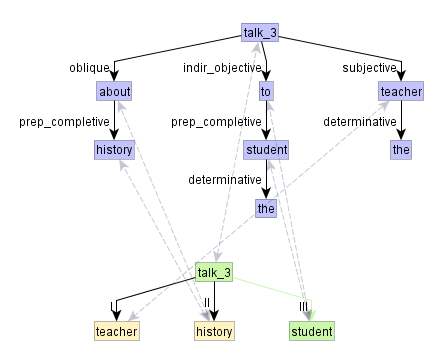
\includegraphics[width=0.5\textwidth, trim = {0cm 0cm 0cm 0cm},clip]{ch6/figs/ssynt.png}
	\caption{Applications des règles actancielles et réalisation des lexies fonctionnelles}
	\label{deroulement4}
\end{figure}

Cela met fin à notre chapitre implémentation. Nous passerons donc à la phase d'évaluation pour vérifier si notre système performe tel que nous l'avions prévu.